\chapter{Oxidação e redução em química orgânica}\label{ch:b1:organic-redox}

Uma garrafa de vinho deixada aberta vira vinagre em poucos dias: bactérias
usam o oxigênio do ar para oxidar o etanol a ácido etanoico. Uma cetona e
o álcool de que ela provém diferem por dois átomos de hidrogênio --- e,
contando direito, por dois elétrons. As oxidações e reduções orgânicas
não se parecem com as trocas de elétrons entre íons metálicos do
\cref{ch:b1:nernst}, porque os elétrons viajam com prótons ou com íons
hidreto, mas a contabilidade é a mesma. Este capítulo atribui \omterm{def:b1:organic-redox:oxidation-level}{níveis de
oxidação} ao carbono, usa-os para prever o que cada álcool dá quando
oxidado e apresenta os reagentes hidretos que reduzem os compostos
carbonílicos, de olho nos grupos que cada reagente deixa intactos.

\begin{recall}
Os \omterm{def:b1:nernst:oxidation-number}{números de oxidação}, as semiequações e o balanceamento das equações
de oxirredução estão no \cref{ch:b1:nernst}; as classes de álcoois e de
carbonos, no \cref{ch:b1:electronic-effects}; os \omterm{def:b1:acetals-protection:hemiacetal}{acetais} e a \omterm{def:b1:acetals-protection:protecting-group}{proteção} dos
grupos carbonila, no \cref{ch:b1:acetals-protection}; as adições de
Grignard, no \cref{ch:b1:organomagnesium}.
\end{recall}

\begin{omfigure}
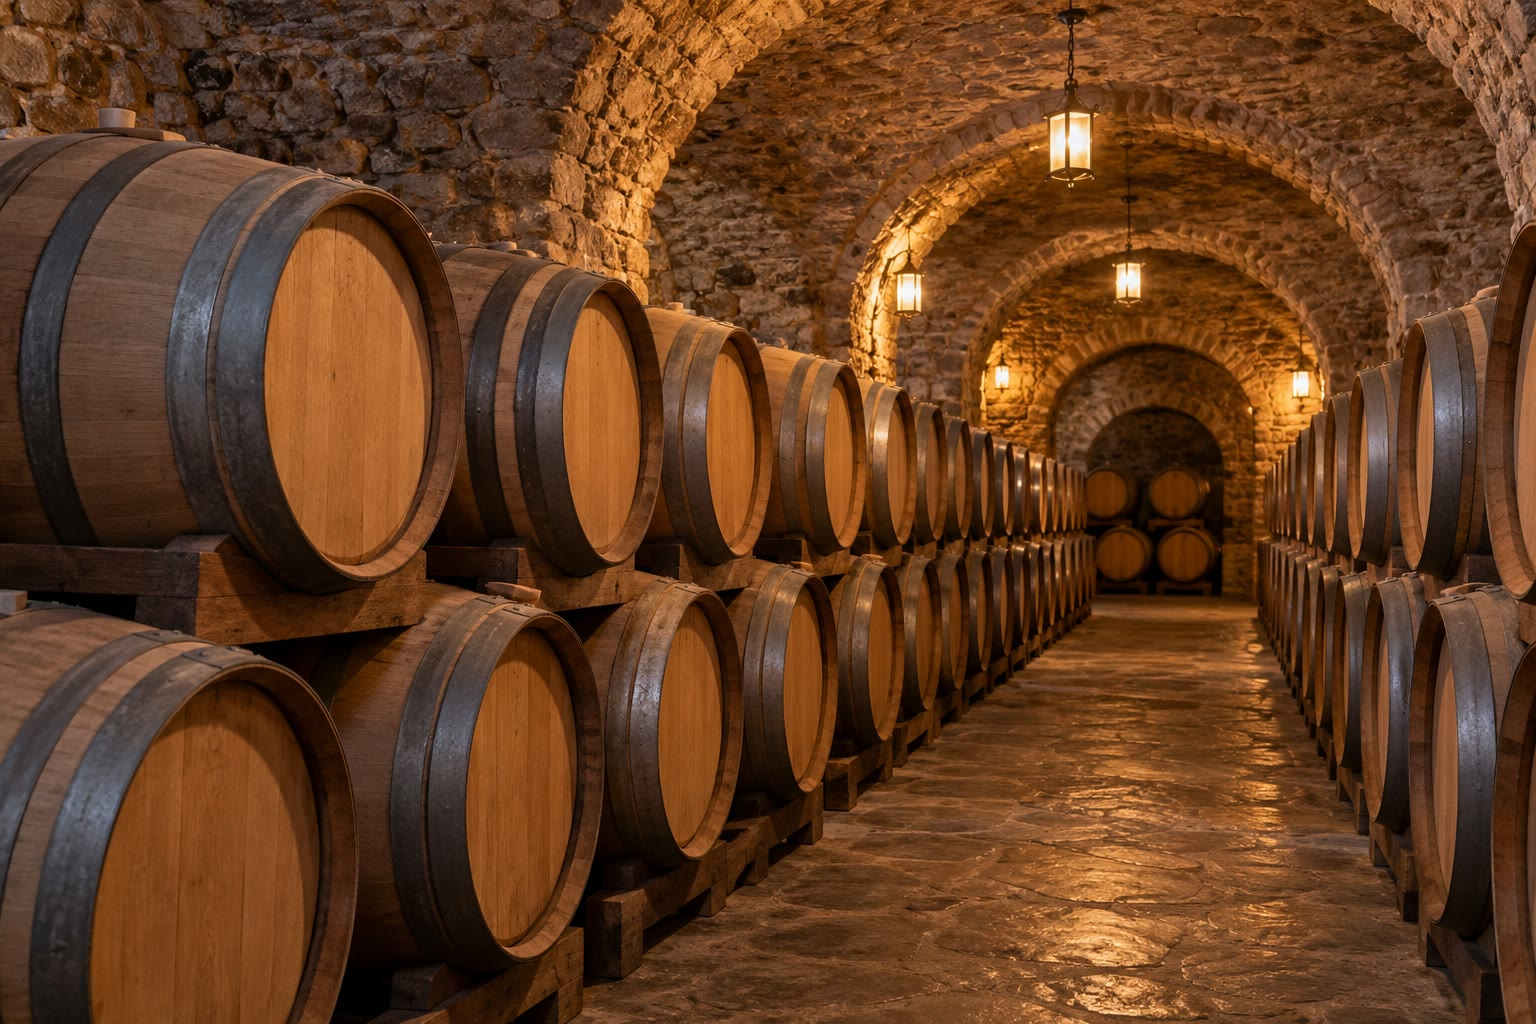
\includegraphics[width=0.58\linewidth]{images/book2/ai/b1-24-wine-cellar.jpg}

{\small Vinho envelhecendo em uma adega. Protegido do ar, o vinho conserva
seu etanol; exposto ao ar, as bactérias acéticas o oxidam a ácido etanoico.}
\end{omfigure}

\section{Níveis de oxidação do carbono}

\begin{definition}[Nível de oxidação]\label{def:b1:organic-redox:oxidation-level}
O \emph{nível de oxidação}\index{nivel de oxidacao@nível de oxidação} de um átomo de carbono é seu
\omterm{def:b1:nernst:oxidation-number}{número de oxidação}, obtido pelas regras da
\cref{prop:b1:nernst:on-rules}: cada ligação com um átomo mais
eletronegativo (O, N, halogênio) conta $+1$, cada ligação com hidrogênio
$-1$, cada ligação com outro carbono 0 (uma ligação dupla conta duas vezes).
\end{definition}

\begin{proposition}[Números de oxidação do carbono]\label{prop:b1:organic-redox:on-of-carbon}
O \omterm{def:b1:nernst:oxidation-number}{número de oxidação} de um carbono é igual a (número de ligações com O, N
ou halogênios) menos (número de ligações com H). Dentro de uma mesma
família de compostos de mesmo esqueleto carbônico, álcool $\to$ aldeído
ou cetona $\to$ ácido carboxílico $\to$ dióxido de carbono é uma série de
oxidações de dois elétrons cada.
\end{proposition}

\begin{proof}
Rompendo cada ligação e dando os dois elétrons ao parceiro mais
eletronegativo: do H (menos eletronegativo que C) o carbono ganha um
elétron, carga $-1$ por C--H; para O, N, halogênios (mais eletronegativos)
ele perde um, $+1$ por ligação; as ligações C--C são divididas igualmente.
Passando de \ce{-CH2OH} ($-1$ para um carbono ligado a um único outro
carbono) a \ce{-CHO} ($+1$) e a \ce{-COOH} ($+3$), o número sobe 2 a cada
etapa: dois elétrons.
\end{proof}

\begin{omfigure}
\begin{tikzpicture}[font=\small, >={Stealth}]
  \foreach \x/\f/\n in {0/\ce{CH4}/-4, 2.4/\ce{CH3OH}/-2, 4.8/\ce{HCHO}/0, 7.2/\ce{HCOOH}/+2, 9.6/\ce{CO2}/+4} {
    \node[draw, rounded corners, minimum width=1.5cm] at (\x,0) {\f};
    \node[below] at (\x,-0.5) {$\n$};
  }
  \foreach \x in {0.8,3.2,5.6,8.0} \draw[->, thick, omThm] (\x,0) -- ++(0.8,0);
  \node[omThm, above] at (4.8,0.5) {oxidação: $-2\,\mathrm{e^-}$ (e $-2\,\ce{H+}$) a cada etapa};
  \node[left] at (-0.9,-0.75) {NO de C:};
\end{tikzpicture}

{\small Os \omterm{def:b1:organic-redox:oxidation-level}{níveis de oxidação} da família de um carbono: metano, metanol,
metanal, ácido metanoico, dióxido de carbono. Cada seta é uma oxidação de
dois elétrons; lida ao contrário, uma redução.}
\end{omfigure}

\begin{method}[Balancear uma semiequação orgânica]\label{met:b1:organic-redox:balance-organic-redox}
\begin{enumerate}
  \item Escreva o \omterm{def:b1:nernst:couple}{oxidante} e o \omterm{def:b1:nernst:couple}{redutor} orgânicos com o mesmo esqueleto.
  \item Conte os elétrons pela variação dos \omterm{def:b1:nernst:oxidation-number}{números de oxidação} dos
        carbonos que mudam (ou simplesmente: dois por par de H perdido, ou
        por O ganho).
  \item Balanceie o oxigênio com água, o hidrogênio com \ce{H+}, a carga
        com os elétrons.
\end{enumerate}
Do etanol ao ácido etanoico: \ce{CH3CH2OH + H2O -> CH3COOH + 4H+ + 4e-}.
Com o dicromato acidificado (\ce{Cr2O7^2- + 14H+ + 6e- -> 2Cr^3+ + 7H2O}),
três moléculas de etanol para dois íons dicromato:
\ce{3CH3CH2OH + 2Cr2O7^2- + 16H+ -> 3CH3COOH + 4Cr^3+ + 11H2O}.
\end{method}

\section{Oxidar os álcoois}

\begin{proposition}[O que os álcoois dão quando oxidados]\label{prop:b1:organic-redox:alcohol-oxidation}
Um álcool primário \ce{RCH2OH} é oxidado ao aldeído \ce{RCHO} e depois
(em água, com um \omterm{def:b1:nernst:couple}{oxidante} forte) ao ácido carboxílico \ce{RCOOH}; um
álcool secundário \ce{R2CHOH}, à cetona \ce{R2CO}, que resiste a uma
oxidação posterior; um álcool terciário \ce{R3COH} não é oxidado sem a
ruptura de uma ligação C--C.
\end{proposition}

\begin{proof}
A oxidação do álcool remove o hidrogênio do OH e um hidrogênio do
carbono carbinólico, formando C=O. Um carbono carbinólico terciário não
tem tal hidrogênio. O aldeído ainda leva um H no carbono carbonílico; em
água, ele é parcialmente hidratado, \ce{RCH(OH)2}, que é oxidado de novo
da mesma maneira a \ce{RCOOH}. Uma cetona não tem H nesse carbono e para.
\end{proof}

Os \omterm{def:b1:nernst:couple}{oxidantes} fortes em água --- dicromato de potássio ou permanganato
acidificados --- oxidam os álcoois primários a ácidos. Para parar no
aldeído, ele é destilado à medida que se forma (os aldeídos fervem a
temperatura mais baixa que os álcoois de que provêm, por não terem
\omterm{def:b1:intermolecular-forces-solvents:hbond}{ligações de hidrogênio} O--H), ou usam-se reagentes mais brandos e
anidros, descritos no volume do 2.º~ano.

\begin{safety}{\ghs[5mm]{GHS03}\,\ghs[5mm]{GHS05}\,\ghs[5mm]{GHS06}\,\ghs[5mm]{GHS07}\,\ghs[5mm]{GHS08}\,\ghs[5mm]{GHS09}}
O dicromato de potássio, o clássico \omterm{def:b1:nernst:couple}{oxidante} alaranjado dos álcoois, é
classificado entre as substâncias que podem causar câncer: só é
manipulado em pequenas quantidades, com luvas e óculos, e seus resíduos
de cromo são recolhidos à parte; sempre que possível, prefere-se um
\omterm{def:b1:nernst:couple}{oxidante} menos perigoso.
% ledger: ghs:K2Cr2O7
\end{safety}

\section{Reduzir os compostos carbonílicos com hidretos}

\begin{definition}[Doador de hidreto]\label{def:b1:organic-redox:hydride-donor}
Um \emph{doador de hidreto}\index{doador de hidreto} transfere um átomo de
hidrogênio com seu \omterm{def:b1:lewis-resonance-vsepr:lewis}{par ligante}, \ce{H-}, a um carbono eletrofílico. O
boro-hidreto de sódio \ce{NaBH4} e o hidreto de lítio e alumínio \ce{LiAlH4} são \emph{hidretos
metálicos complexos}\index{hidreto metalico complexo@hidreto metálico complexo}: o hidreto é entregue
a partir do íon \ce{BH4-} ou \ce{AlH4-}, não como íon livre.
\end{definition}

\begin{omfigure}
\setchemfig{atom sep=2.1em}
\schemestart
\chemfig{H_3B^{-}-[@{bh}]@{h}H}
\+
\chemfig{@{c}C(-[:150]R)(-[:210]R')=[@{co}]@{o}O}
\arrow{->}
\chemfig{C(-[:150]R)(-[:210]R')(-[2]H)-O^{-}}
\arrow{->[\ce{H2O}]}
\chemfig{C(-[:150]R)(-[:210]R')(-[2]H)-OH}
\schemestop
\chemmove{\draw[->, thick, shorten <=2pt, shorten >=3pt](bh) .. controls +(80:9mm) and +(180:7mm) .. (c);
          \draw[->, thick, shorten <=2pt, shorten >=2pt](co) .. controls +(90:6mm) and +(90:6mm) .. (o);}
\par\vspace{6pt}

{\small Redução de uma cetona pelo boro-hidreto: um par B--H forma a nova
ligação C--H enquanto o par $\pi$ da C=O vai para o oxigênio; o \omterm{def:b1:alcohol-activation:alkoxide}{alcóxido} é
protonado pelo solvente (água ou um álcool) ou no tratamento. Cada
\ce{BH4-} pode entregar seus quatro hidrogênios, um após o outro.}
\end{omfigure}

\begin{proposition}[Alcance dos dois hidretos]\label{prop:b1:organic-redox:hydride-scope}
O boro-hidreto de sódio, usado em água ou em álcoois, reduz os aldeídos a
álcoois primários e as cetonas a álcoois secundários, e deixa intactos
os ésteres, os ácidos carboxílicos, as amidas e as ligações duplas C=C. O
hidreto de lítio e alumínio, usado em éter seco, reduz também os ésteres
e os ácidos carboxílicos a álcoois primários, e reage violentamente com a água.
\end{proposition}

\begin{proof}
A ligação Al--H é mais polarizada que a ligação B--H (o alumínio é menos
eletronegativo que o boro), de modo que \ce{AlH4-} é um \omterm{def:b1:organic-redox:hydride-donor}{doador de hidreto}
muito mais forte, capaz de atacar a carbonila menos eletrofílica dos
ésteres e dos carboxilatos; a mesma reatividade o faz reagir com qualquer
hidrogênio ácido, inclusive o da água. \ce{BH4-} reage só lentamente com
a água e os álcoois, e ataca apenas as carbonilas mais eletrofílicas. Uma
ligação C=C isolada não é eletrofílica e não é reduzida por nenhum dos dois.
\end{proof}

\section{Seletividade}

\begin{definition}[Reação quimiosseletiva]\label{def:b1:organic-redox:chemoselective}
Uma \emph{reação quimiosseletiva}\index{reacao quimiosseletiva@reação quimiosseletiva} age
sobre um grupo funcional de uma molécula na presença de outros que
poderiam, com outro reagente, reagir também.
\end{definition}

\begin{omfigure}
\begin{tabular}{lcc}
\hline
grupo & \ce{NaBH4} (solvente álcool) & \ce{LiAlH4} (éter seco) \\
\hline
aldeído \ce{RCHO} & álcool primário & álcool primário \\
cetona \ce{R2CO} & álcool secundário & álcool secundário \\
éster \ce{RCOOR} & sem reação & dois álcoois \\
ácido carboxílico \ce{RCOOH} & sem reação (sal) & álcool primário \\
alceno \ce{C=C} & sem reação & sem reação \\
\omterm{def:b1:acetals-protection:hemiacetal}{acetal} & sem reação & sem reação \\
\hline
\end{tabular}

\smallskip
{\small O que os dois hidretos reduzem. O boro-hidreto de sódio é o
reagente quimiosseletivo; o hidreto de lítio e alumínio, o poderoso.}
\end{omfigure}

\begin{example}[Um cetoéster]\label{ex:b1:organic-redox:ketoester}
O 4-oxopentanoato de etila, \ce{CH3CO(CH2)2COOEt}, com o boro-hidreto de
sódio dá o 4-hidroxipentanoato de etila: só a cetona é reduzida. Com o
hidreto de lítio e alumínio, os dois grupos são reduzidos: pentano-1,4-diol
(e etanol). Para reduzir só o éster, a cetona precisa antes ser protegida
como \omterm{def:b1:acetals-protection:hemiacetal}{acetal} (\cref{ch:b1:acetals-protection}).
\end{example}

\begin{inthelab}[Reduzir uma cetona]
O boro-hidreto de sódio é adicionado em pequenas porções a uma solução
fria da cetona em etanol: a reação é exotérmica, e o hidrogênio borbulha
devido à lenta reação do reagente com o solvente. Após a agitação, um
ácido diluído destrói o excesso de reagente (mais hidrogênio: nenhuma
chama por perto) e o álcool é extraído. O hidreto de lítio e alumínio,
ao contrário, só é usado em éter seco sob gás inerte, e seu excesso é
destruído com muito cuidado.
\end{inthelab}

\section{Exercícios}

\begin{exercise}[$\star$]\label{exo:b1:organic-redox:1}
Dê o \omterm{def:b1:nernst:oxidation-number}{número de oxidação} de cada carbono no etanol, no etanal, no ácido
etanoico, na propanona e no ácido metanoico.
\end{exercise}

\begin{exercise}[$\star$]\label{exo:b1:organic-redox:2}
O que o dicromato acidificado dá com o propan-1-ol, o propan-2-ol e o
2-metilpropan-2-ol?
\end{exercise}

\begin{exercise}[$\star$]\label{exo:b1:organic-redox:3}
Escreva as semiequações dos pares propanona/propan-2-ol e
etanal/etanol em meio ácido.
\end{exercise}

\begin{exercise}[$\star$]\label{exo:b1:organic-redox:4}
O que o boro-hidreto de sódio e o hidreto de lítio e alumínio dão com o
butanal, a butanona, o butanoato de etila e o ácido butanoico?
\end{exercise}

\begin{exercise}[$\star\star$]\label{exo:b1:organic-redox:5}
Balanceie a oxidação do propan-2-ol pelo permanganato em meio ácido
(\ce{MnO4-}/\ce{Mn^2+}) e calcule o volume de permanganato a
\qty{0.020}{mol/L} necessário para \qty{1.20}{g} de álcool ($M = \qty{60.0}{g/mol}$).
\end{exercise}

\begin{exercise}[$\star\star$]\label{exo:b1:organic-redox:6}
Como obter propanal a partir do propan-1-ol sem que ele seja oxidado
além disso? Use as temperaturas de ebulição: propan-1-ol \qty{97}{\celsius}, propanal
\qty{48}{\celsius}.
% ledger: bp:propanal, bp:propan-1-ol
\end{exercise}

\begin{exercise}[$\star\star$]\label{exo:b1:organic-redox:7}
Escreva o mecanismo da redução do etanal por \ce{BH4-} em etanol.
Que átomo do produto vem do reagente?
\end{exercise}

\begin{exercise}[$\star\star$]\label{exo:b1:organic-redox:8}
A redução da butan-2-ona com \ce{NaBH4} dá um álcool \omterm{def:b1:stereochemistry-in-depth:stereocentre}{quiral}. Ele é
opticamente ativo? Por quê?
\end{exercise}

\begin{exercise}[$\star\star$]\label{exo:b1:organic-redox:9}
No teste do bafômetro usado antigamente pela polícia, o dicromato
alaranjado ficava verde. Escreva a reação com o etanol e explique a
mudança de cor.
\end{exercise}

\begin{exercise}[$\star\star\star$]\label{exo:b1:organic-redox:10}
Proponha sínteses de: 2-metilbutan-2-ol a partir do etanal e de um
\omterm{def:b1:organomagnesium:organometallic}{reagente de Grignard}, seguido de uma oxidação e de uma segunda etapa de
Grignard; pentan-3-ol a partir do propanal. Conte as oxidações e as reduções.
\end{exercise}

\begin{exercise}[$\star\star\star$]\label{exo:b1:organic-redox:11}
Reduza apenas o grupo éster do 4-oxopentanoato de metila,
\ce{CH3CO(CH2)2COOCH3}. Planeje as três etapas com uma \omterm{def:b1:acetals-protection:protecting-group}{proteção} e dê o
produto.
\end{exercise}

\begin{exercise}[$\star\star\star$]\label{exo:b1:organic-redox:12}
Mostre que, na oxidação de um álcool primário a ácido, quatro elétrons
são trocados, pelos \omterm{def:b1:nernst:oxidation-number}{números de oxidação} e pela semiequação. Generalize
para a oxidação do metano a dióxido de carbono.
\end{exercise}

\section{Problema: do ciclo-hexanol ao ácido adípico}

\begin{problem}[{Problema de fim de semana --- os níveis de oxidação no
ciclo-hexanol, na ciclo-hexanona e no ácido adípico, a oxidação nítrica e
seus elétrons, uma rota com peróxido de hidrogênio, e a massa de óxido de
dinitrogênio liberada por tonelada de ácido adípico}]
\label{pb:b1:organic-redox:1}
O ácido adípico, ácido hexanodioico \ce{HOOC(CH2)4COOH}, é produzido em
grande escala para os náilons, sobretudo pela oxidação do ciclo-hexanol
(com a ciclo-hexanona) pelo ácido nítrico, que libera óxido de
dinitrogênio \ce{N2O}, um potente gás de efeito estufa. Massas molares (\unit{g/mol}): \ce{C6H12O} 100.0,
\ce{C6H10O} 98.0, \ce{C6H10O4} 146.0, \ce{N2O} 44.0, \ce{HNO3} 63.0,
\ce{H2O2} 34.0.

\medskip
\noindent\textbf{Parte I --- \omterm{def:b1:organic-redox:oxidation-level}{Níveis de oxidação}.}
\begin{enumerate}
  \item Dê o \omterm{def:b1:nernst:oxidation-number}{número de oxidação} de cada carbono do ciclo-hexanol.
  \item O mesmo para a ciclo-hexanona.
  \item O mesmo para o ácido adípico.
  \item Quais carbonos são oxidados na passagem do ciclo-hexanol ao ácido
        adípico, e que ligação é rompida?
  \item Quantos elétrons uma molécula de ciclo-hexanol perde?
  \item Por que a ciclo-hexanona, uma cetona, é ainda assim oxidada aqui?
\end{enumerate}

\medskip
\noindent\textbf{Parte II --- A rota do ácido nítrico.}
\begin{enumerate}[resume]
  \item Escreva a semiequação do ciclo-hexanol ao ácido adípico em meio ácido.
  \item Dê o \omterm{def:b1:nernst:oxidation-number}{número de oxidação} de N em \ce{HNO3} e em \ce{N2O}.
  \item Escreva a semiequação \ce{HNO3}/\ce{N2O}.
  \item Combine-as; verifique que se obtém
        \ce{C6H12O + 2HNO3 -> C6H10O4 + N2O + 2H2O}.
  \item Quantos mols de elétrons são trocados por mol de ácido
        adípico?
  \item Calcule a massa de ácido nítrico consumida por tonelada de ácido adípico.
\end{enumerate}

\medskip
\noindent\textbf{Parte III --- Uma rota com peróxido de hidrogênio.}
\begin{enumerate}[resume]
  \item Escreva a semiequação \ce{H2O2}/\ce{H2O}.
  \item Escreva e balanceie a oxidação do ciclo-hexanol pelo peróxido de
        hidrogênio a ácido adípico.
  \item Calcule a massa de \ce{H2O2} por tonelada de ácido adípico.
  \item Qual é o único subproduto? Por que essa rota é chamada de mais verde?
  \item O peróxido de hidrogênio precisa ser ativado por um \omterm{def:b1:elementary-steps:catalyst}{catalisador}.
        Usando o \cref{exo:b1:nernst:12}, explique por que uma oxidação
        termodinamicamente favorecida ainda pode precisar de um.
  \item O que o boro-hidreto de sódio faria com a ciclo-hexanona? Escreva a
        reação.
\end{enumerate}

\medskip
\noindent\textbf{Parte IV --- Massas e o gás de efeito estufa.}
\begin{enumerate}[resume]
  \item Calcule a quantidade de matéria de ácido adípico em uma tonelada.
  \item Calcule a quantidade de \ce{N2O} formada com ela pela rota nítrica.
  \item Calcule a massa de ciclo-hexanol necessária por tonelada, com
        \qty{95}{\percent} de \omterm{def:b1:extent-q-and-k:fractional-extent}{rendimento}.
  \item Indique a massa de \ce{N2O} liberada por tonelada de ácido adípico
        pela rota nítrica, em toneladas.
\end{enumerate}
\end{problem}
